\documentclass[conf]{new-aiaa}
%\documentclass[journal]{new-aiaa} for journal papers
\usepackage[utf8]{inputenc}

\usepackage{graphicx}
\usepackage{amsmath}
\usepackage[version=4]{mhchem}
\usepackage{siunitx}
\usepackage{longtable,tabularx}
\setlength\LTleft{0pt} 
\usepackage{caption}
\usepackage{subcaption}

\title{DP0: Control of a platform with a reaction wheel in gravity}

\author{Timothy Bretl}
\affil{University of Illinois at Urbana-Champaign}

\begin{document}

\maketitle

\begin{abstract}
%In this report, we design a controller to stabilize a rotating platform with a reaction wheel in gravity at an inverted configuration, and test this controller with experiments in simulation.
%In particular, we applied eigenvalue placement to design 
In this report, we design a controller to stabilize an inverted rotating platform with a reaction wheel in gravity, and test this controller with experiments in simulation. We linearize equations of motion to derive a state-space model and apply eigenvalue placement to choose linear state feedback that would, in theory, produce a stable closed-loop system that achieves target values of peak time and peak overshoot. Our experiments show that we achieved a 30\% smaller peak time and a 120\% larger peak overshoot than intended, and that stable closed-loop responses were obtained only when starting from initial conditions close to equilibrium.
\end{abstract}

\section{Nomenclature}

{\renewcommand\arraystretch{1.0}
\noindent\begin{longtable*}{@{}l @{\quad=\quad} l@{}}
$A, B$ & matrices that describe the state-space model \\
$J_{1}, J_{2}$  & moments of inertia of the platform and wheel ($\text{kg}\cdot\text{m}^{2}$) \\
$K$ ($k_{1}, k_{2}, k_{3}$) & gain matrix (and the three elements of this matrix) for linear state feedback \\
$l$& distance from center of platform to center of wheel (m) \\
$m, g$ & mass of wheel (kg) and acceleration of gravity ($\text{m}/\text{s}^{2}$) \\
%$m$ &    mess of wheel (kg) \\
$q_{1e}, v_{1e}, v_{2e}, \tau_{e}$ & equilibrium values of nonlinear states and inputs \\
$q_{1}, v_{1}, v_{2}$ & platform angle (rad) platform angular velocity (rad/s), and wheel angular velocity (rad/s)\\
%$t$ & time (s) \\
$\tau$ & torque applied by wheel to platform ($\text{N}\cdot\text{m}$) \\
$T_{p}, M_{p}$ & peak time (s) and peak overshoot \\
$x, u$ & state and input of linear system \\
$\zeta, \mu$ & state and input of nonlinear system \\
\end{longtable*}}


\section{Introduction}
\lettrine{C}{onsider} an inverted platform in a gravitational field that is constrained to rotate about one axis and to which is mounted a reaction wheel (Fig.~\ref{fig-snapshot}). Suppose it is possible to measure the platform angle, the platform angular velocity, and the wheel angular velocity, and to choose a torque that is applied by the platform to the wheel. Our goal is to design a controller that stabilizes the inverted platform (and that maintains the wheel at some non-zero velocity)---in particular, at a configuration that would otherwise be unstable. This challenge is representative of what we might see when designing attitude determination and control systems for spacecraft in low Earth orbit that use gravity gradient torques to dump momentum \cite{Markley2014}. Section \ref{sec-theory} derives a state-space model of our system by linearizing about an equilibrium point and then applies eigenvalue placement to design linear state feedback that would achieve target peak time and peak overshoot, which are common step response specifications \cite{Astrom2021}.
Section \ref{sec-methods} describes how we implemented and tested our controller in simulation, and in particular describes the experiments we conducted to quantify the extent to which target values of peak time and peak overshoot were achieved as well as the experiments we conducted to identify the {\em basin of attraction}---the set of initial conditions from which the closed-loop system is stable in simulation. Section \ref{sec-results} presents the results of these experiments.
Section \ref{sec-conclusion} concludes with opportunities for future work.


\section{Theory}
\label{sec-theory}

\subsection{Derive state-space model}
\label{sec-model}

The motion of the platform and wheel together under gravity is described by
\begin{equation}
\begin{aligned}
J_1 \ddot{q}_1 &= \tau - mgl\sin(q_1) \\
J_2 \dot{v}_2 &= - \left( \dfrac{J_1 + J_2}{J_1} \right) \tau + \left( \dfrac{J_2}{J_1} \right) mgl\sin(q_1),
\end{aligned}
\label{eq-eom}
\end{equation}
where $q_{1}$ is the angle of the platform, $v_{2}$ is the angular velocity of the wheel, $\tau$ is the torque applied by the platform to the wheel through a motor, and all other parameters are given constants.
Before proceeding with control design, we will linearize these equations of motion about an equilibrium point that corresponds to some desired platform angle.
First, we rewrite \eqref{eq-eom} as a set of three first-order ordinary differential equations
\begin{equation}
\begin{aligned}
\dot{q}_{1} &= v_{1} \\
\dot{v}_{1} &= \left( \tau - mgl\sin(q_1) \right) / J_{1} \\
\dot{v}_{2} &= - \left( (J_1 + J_2) \tau + ( J_{2} mgl\sin(q_1) \right) / (J_{1}J_{2}),
\end{aligned}
\label{eq-eom-firstorder}
\end{equation}
where we have introduced a variable $v_{1}$ to denote the angular velocity of the platform. If we define
\begin{equation}
\zeta = \begin{bmatrix} q_{1} \\ v_{1} \\ v_{2} \end{bmatrix}
\qquad\qquad
\mu = \begin{bmatrix} \tau \end{bmatrix}
\end{equation}
then we can rewrite \eqref{eq-eom-firstorder} in the general form
\begin{equation}
\dot{\zeta} = f(\zeta, \mu) =
\begin{bmatrix}
v_{1} \\
\left( \tau - mgl\sin(q_1) \right) / J_{1} \\
- \left( (J_1 + J_2) \tau + ( J_{2} mgl\sin(q_1) \right) / (J_{1}J_{2})
\end{bmatrix}.
\label{eq-eom-general}
\end{equation}
By solving
\begin{equation}
0 = f(\zeta_{e}, \mu_{e}),
\end{equation}
we see that any equilibrium point of \eqref{eq-eom-general} has the form
\begin{equation}
\zeta_{e} = \begin{bmatrix} n\pi \\ 0 \\ v_{2e} \end{bmatrix}
\qquad\qquad
\mu_{e} = \begin{bmatrix} 0 \end{bmatrix}
\end{equation}
for some integer $n \in \mathbb{Z}$ and some choice of wheel velocity $v_{2e} \in \mathbb{R}$. Recognizing that the angles $n\pi$ and $(n+2)\pi$ correspond to the same orientation of the platform for any $n$, we restrict our choice of equilibrium platform angle to either $0\;\text{radians}$ or $\pi\;\text{radians}$. Of these two, since we would like to consider what seems to be the more challenging case of stabilizing the platform at an inverted configuration, we choose $\pi\;\text{radians}$ as the equilibrium platform angle. Since reaction wheels are typically designed to operate most efficiently at non-zero angular velocity, we choose
\begin{equation}
v_{2e} = 50\;\text{rpm} = 5\pi/3\;\text{radians}/\text{second}
\end{equation}
and so arrive at
\begin{equation}
\zeta_{e} = \begin{bmatrix} \pi \\ 0 \\ 5\pi/3 \end{bmatrix}
\qquad\qquad
\mu_{e} = \begin{bmatrix} 0 \end{bmatrix}.
\end{equation}
If we define
\begin{equation}
x = \zeta - \zeta_{e}
\qquad\qquad
u = \mu - \mu_{e},
\end{equation}
then \eqref{eq-eom-general} can be approximated close to the equilibrium point by the linear system
\begin{equation}
\dot{x} = Ax+Bu
\label{eq-ss}
\end{equation}
where
\begin{equation}
A
= \frac{\partial f}{\partial \zeta}\biggr\rvert_{\zeta_{e}, \mu_{e}}
= \begin{bmatrix} 0 & 1 & 0 \\ mgl/J_{1} & 0 & 0 \\ -mgl/J_{1} & 0 & 0 \end{bmatrix}
\qquad\qquad
B
= \frac{\partial f}{\partial \mu}\biggr\rvert_{\zeta_{e}, \mu_{e}}
= \begin{bmatrix} 0 \\ 1/J_{1} \\ -(J_{1} + J_{2}) / (J_{1}J_{2}) \end{bmatrix}.
\end{equation}


\subsection{Design linear state feedback}
\label{sec-design}

Suppose we choose to apply an input of the form
\begin{equation}
u = - Kx
\end{equation}
where
\begin{equation}
K = \begin{bmatrix} k_{1} & k_{2} & k_{3} \end{bmatrix}
\end{equation}
for some choice of gains $k_{1}$, $k_{2}$, and $k_{3}$. The resulting closed-loop system is
\begin{equation}
\dot{x} = (A - BK) x.
\label{eq-closedloop}
\end{equation}
We will choose gains by eigenvalue placement, applying a common heuristic to choose desired closed-loop eigenvalue locations that achieve given step response specifications\cite{Astrom2021}.
In particular, suppose we want the closed-loop response to a unit disturbance in the platform angle to have a peak time $T_{p}$ and peak overshoot $M_{p}$ of about
\begin{equation}
T_{p} = \pi / 4 \approx 0.8\;\text{seconds}
\qquad\qquad
M_{p} = e^{-\pi / 2} \approx 0.2.
\label{eq-peaktargets}
\end{equation}
If the system were second-order, we could achieve these specifications by placing eigenvalues at $-\sigma \pm j\omega$ where
\begin{equation}
\sigma = -\ln(M_{p}) / T_{p} = 2
\qquad\qquad
\omega = \pi / T_{p} = 4.
\label{eq-heuristic}
\end{equation}
We place the third eigenvalue at $-5\sigma$ so that it has a small effect on the closed-loop response relative to these two dominant eigenvalues (i.e., so that the part of the response associated with this third eigenvalue decays much more quickly). In summary, the desired eigenvalue locations are as follows:
\begin{equation}
s_{1} = -2+4j
\qquad\qquad
s_{2} = -2-4j
\qquad\qquad
s_{3} = -10.
\label{eq-eigs}
\end{equation}
The characteristic polynomial that would produce these eigenvalues is
\begin{equation}
(s - s_{1}) (s - s_{2})(s - s_{3}) = s^{3} + 14 s^{2} + 60 s + 200.
\label{eq-charpoly-want}
\end{equation}
The characteristic polynomial of the closed-loop system, as a function of the gains $k_{1}$, $k_{2}$, and $k_{3}$, is
\begin{equation}
s^{3} + \left((-J_{1}k_{3} + J_{2}k_{2} - J_{2}k_{3})/(J_{1}J_{2})\right)s^{2} + \left((k_{1}-mgl)/J1\right)s + mglk_{3}/(J_{1}J_{2}).
\label{eq-charpoly-have}
\end{equation}
Equating coefficients of \eqref{eq-charpoly-want} and \eqref{eq-charpoly-have}, we find
\begin{equation}
k_{1} = mgl + 60J_{1}
\qquad\qquad
k_{2} = 200J_{1}\left(\frac{J_{1} + J_{2}}{mgl} \right) + 14J_{1}
\qquad\qquad
k_{3} = \frac{100J_{1}J_{2}}{mgl}.
\end{equation}
We emphasize that the resulting closed-loop system is asymptotically stable by construction, since all three eigenvalues \eqref{eq-eigs} placed by these gains have negative real part.





\section{Experimental methods}
\label{sec-methods}

\subsection{Control implementation and simulation architecture}

We verified our control design with experiments in simulation.
The simulator itself already existed and was implemented using PyBullet\cite{coumans2021}.
We added a python-based implementation of our controller, starting from template code that was provided with the simulator\cite{ae353software}.
In particular, this controller did the following things at a rate of 100 Hz:
\begin{itemize}

\item It received measurements of the platform angle, the platform angular velocity, and the wheel angular velocity from the simulator (along with the current time, which we did not use).

\item It computed the state $x$ from these measurements, given our choice of equilibrium point (Section \ref{sec-model}).

\item It computed the input $u$ from $x$ by application of linear state feedback (Section \ref{sec-design}).

\item It computed the torque $\tau$ from $u$, again given our choice of equilibrium point (Section \ref{sec-model}).

\item It sent the wheel torque command $-\tau$ to the simulator, where the change in sign was due to our having chosen to define $\tau$ as the torque applied by the wheel to the platform, while the simulator expected the controller to specify the equal and opposite torque applied by the platform to the wheel.

\end{itemize}
Each experiment began at initial conditions---initial values of the platform angle, the platform angular velocity, and the wheel angular velocity---that we chose, and lasted five seconds of simulation time. Both our controller and the simulator were deterministic, so the results of an experiment were always the same if repeated from the same initial conditions. Data produced by each experiment were a time-history (at 100 Hz) of the platform angle, the platform angular velocity, the wheel velocity, the commanded wheel torque, and the actual wheel torque after saturation at torque limits.

\subsection{Experiments to find peak time and peak overshoot}
\label{sec-peak}

We had designed our controller to achieve a peak time of approximately $0.80\;\text{seconds}$ and a peak overshoot of approximately $0.20$, starting from a unit disturbance in the platform angle. To quantify the extent to which this goal was met, we conducted a single experiment with the following initial conditions:
\begin{equation}
q_{1}(0) = q_{1e} + 0.1 = \pi + 0.1
\qquad\qquad
v_{1}(0) = v_{1e} = 0
\qquad\qquad
v_{2}(0) = v_{2e} = 5\pi/3
\label{eq-peak-ics}
\end{equation}
These initial conditions correspond to starting with an initial error in platform angle of $0.1\;\text{radians}$ and with zero initial error in platform angular velocity and wheel angular velocity.
Starting from these initial conditions, we computed the {\em peak time} as the first non-zero time $T_{p}$ at which the platform angle reaches a local minimum (i.e., stops decreasing and starts increasing again).
We computed the {\em peak overshoot} as the fraction
\begin{equation}
M_{p} = \left\lvert\frac{q_{1}(T_{p}) - q_{1e}}{q_{1}(0) - q_{1e}}\right\rvert,
\end{equation}
in other words as the error in platform angle at the peak time, normalized by the initial error in platform angle.

\subsection{Experiments to find the basin of attraction}
\label{sec-basin}

We had designed our controller to make the linear system \eqref{eq-ss} asymptotically stable in closed loop. In theory, this would imply that $x(t) \rightarrow 0$ as $t \rightarrow \infty$ for any set of initial conditions $x(0)$. In practice, however, the model \eqref{eq-ss} is only valid near the equilibrium point about which we linearized. For this reason, we conducted a set of experiments to find the {\em basin of attraction}---that is, to find the set of initial conditions from which the closed-loop system converges to equilibrium (within some reasonable amount of time) in simulation.
We assumed that $v_{2}(0) = v_{2e}$ for all of these experiments and restricted our attention only to changes in the initial platform angle $q_{1}(0)$ and angular velocity $v_{1}(0)$.
These initial conditions were said to be inside the basin of attraction when the resulting trajectory satisfied
\begin{equation}
\left.\begin{matrix}
|q_{1}(t) - q_{1e}| < 0.01 \\
|v_{1}(t) - v_{1e}| < 0.01 \\
|v_{2}(t) - v_{2e}| < 0.01
\end{matrix}
\right\}
\;\text{for all}\; t \in [4, 5].
\label{eq-stablecond}
\end{equation}
We found points on the boundary of the basin of attraction by searching along rays in the space of initial errors in platform angle and angular velocity.
In particular, for each $n_{\theta} \in \{0, 1, 2, \ldots, 100 \}$
we found the smallest $n_{d} \in \{0, 1, 2, \ldots\}$
for which the initial conditions
\begin{equation}
q_{1}(0) = q_{1e} + (\delta n_{d})\cos\left(2\pi n_{\theta} / 100\right)
\qquad\qquad
v_{1}(0) = v_{1e} + (\delta n_{d})\sin\left(2\pi n_{\theta} / 100\right)
\qquad\qquad
v_{2}(0) = v_{2e}
\end{equation}
did {\em not} produce a trajectory satisfying \eqref{eq-stablecond}, and added that point to our boundary.


\section{Results and discussion}
\label{sec-results}

\begin{figure}[p]
\centering
\begin{subfigure}[t]{0.49\textwidth}
\centering
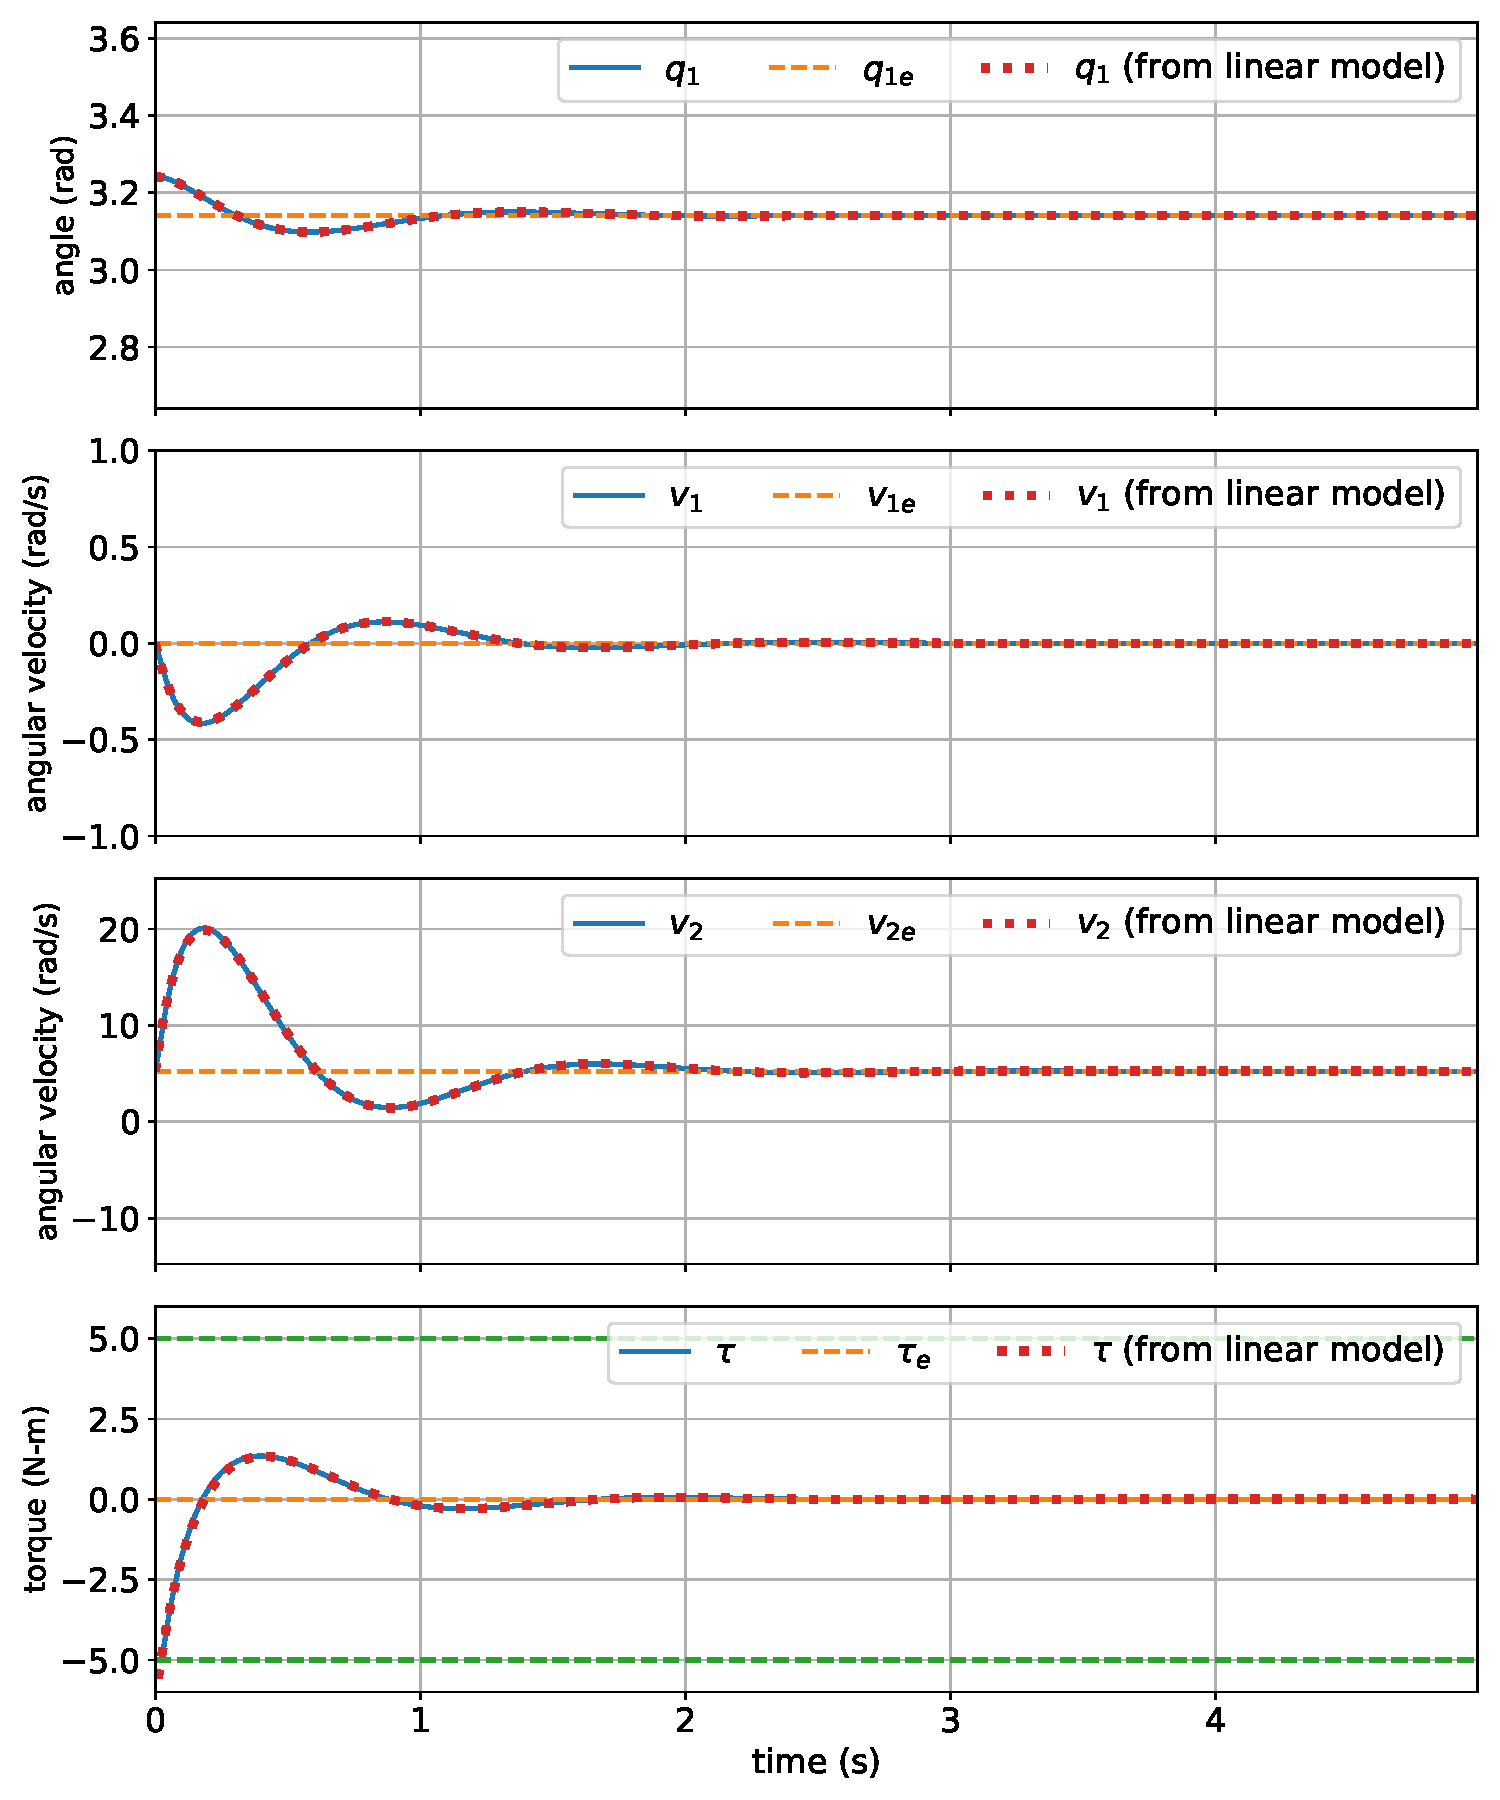
\includegraphics[width=\textwidth]{fig01}
\caption{An example of {\em stable} closed-loop response in simulation (i.e., states {\em do} converge to equilibrium within four seconds), with an initial error in platform angle of $0.1\;\text{rad}$ and with zero initial error in both platform angular velocity and wheel angular velocity.}
\label{fig-stable}
\end{subfigure}
\hfill
\begin{subfigure}[t]{0.49\textwidth}
\centering
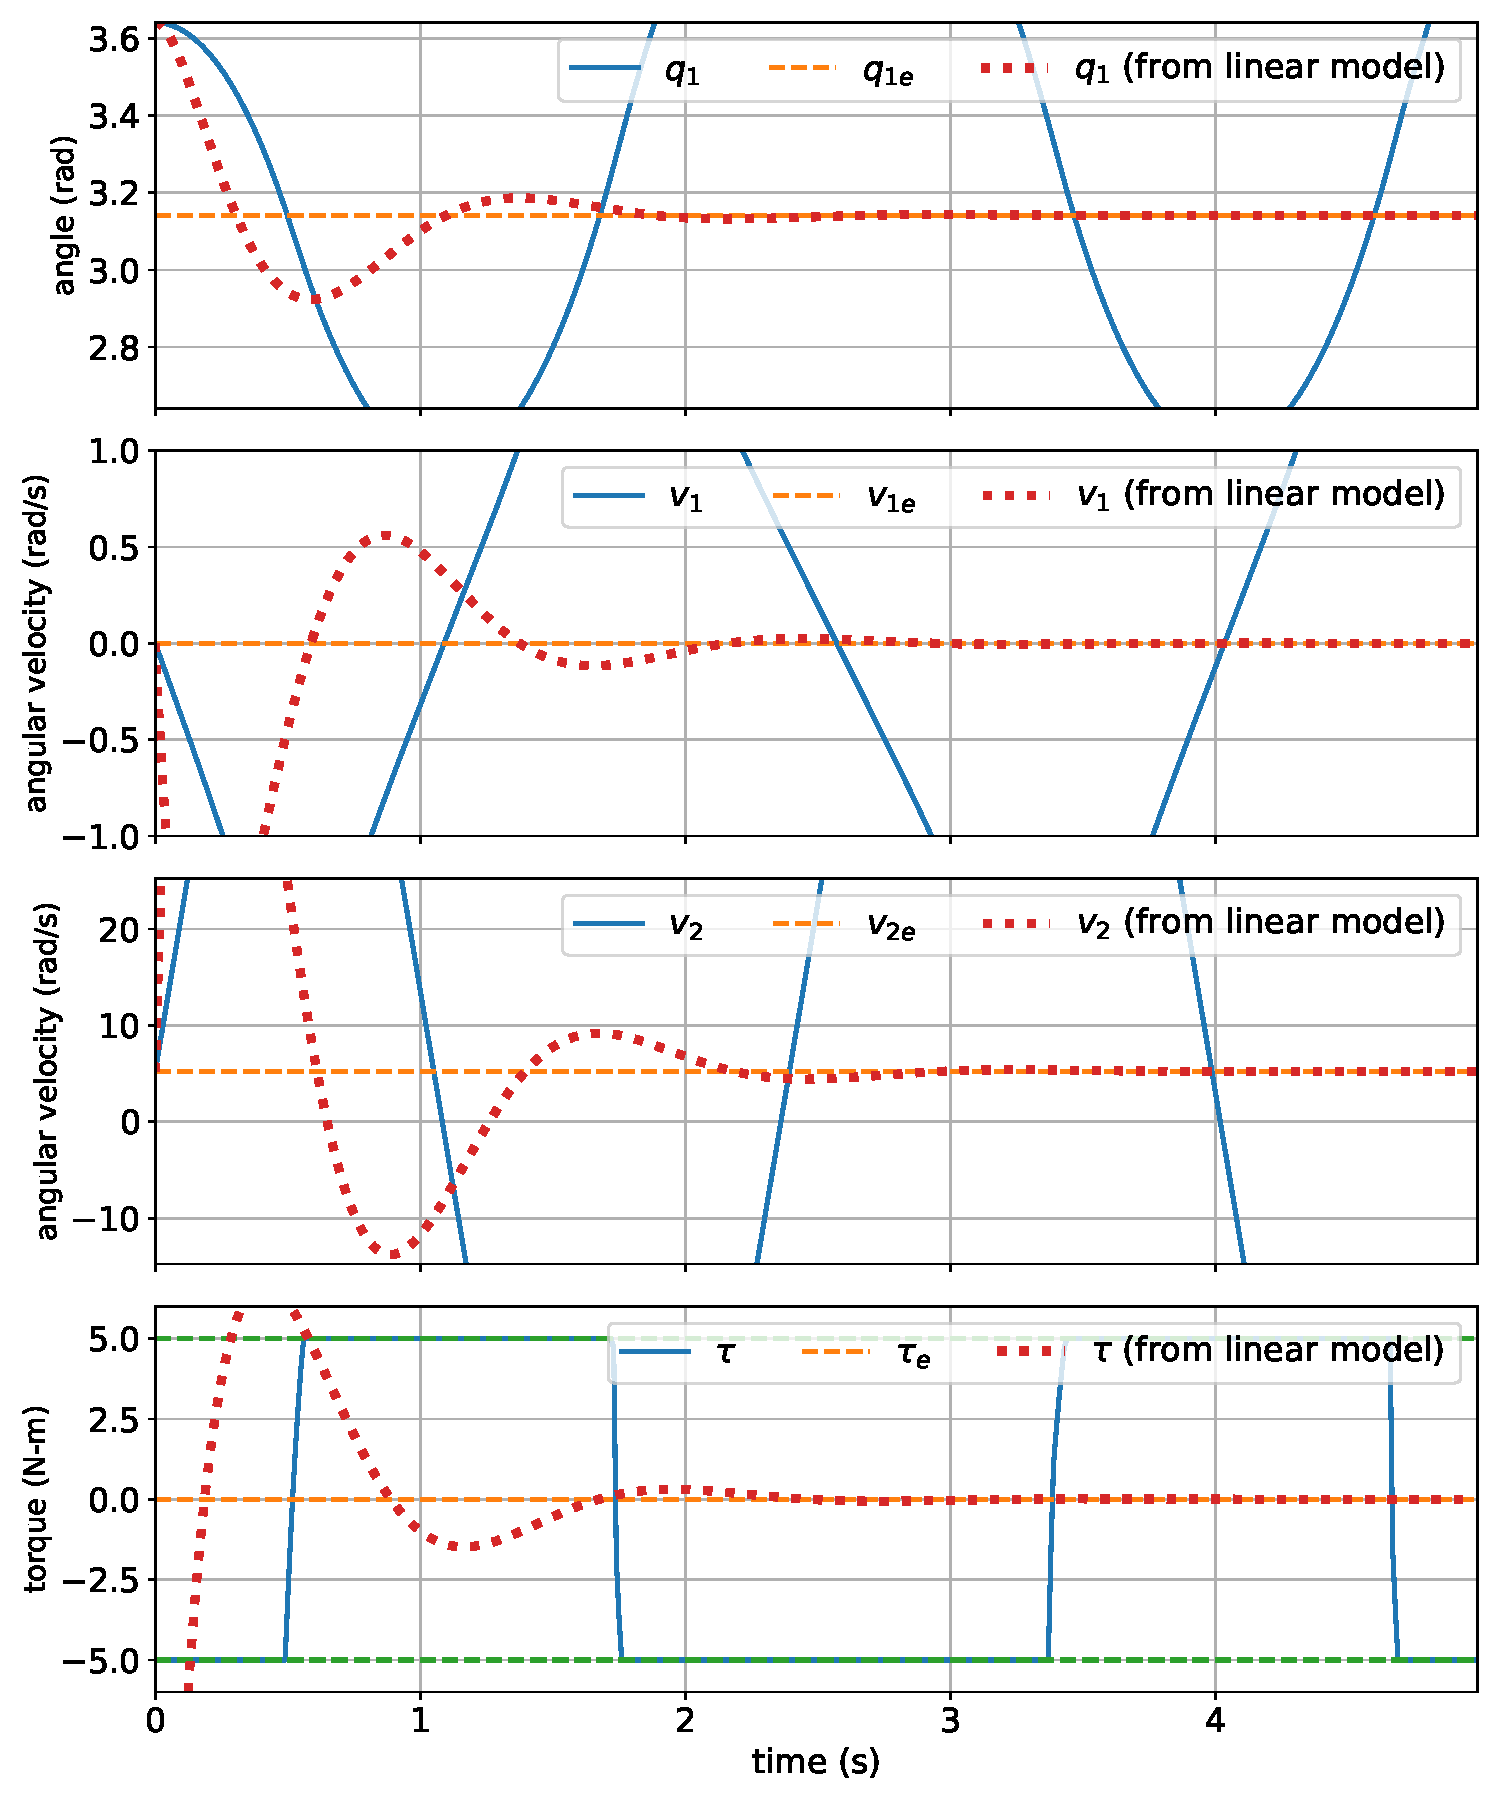
\includegraphics[width=\textwidth]{fig02}
\caption{An example of {\em unstable} closed-loop response in simulation (i.e., states do {\em not} converge to equilibrium within four seconds), with an initial error in platform angle of $0.5\;\text{rad}$ and with zero initial error in both platform angular velocity and wheel angular velocity.}
\label{fig-unstable}
\end{subfigure}
\caption{Examples of stable and unstable closed-loop responses in simulation.}
\label{fig-examples}
\end{figure}

%\begin{figure}[p]
%\centering
%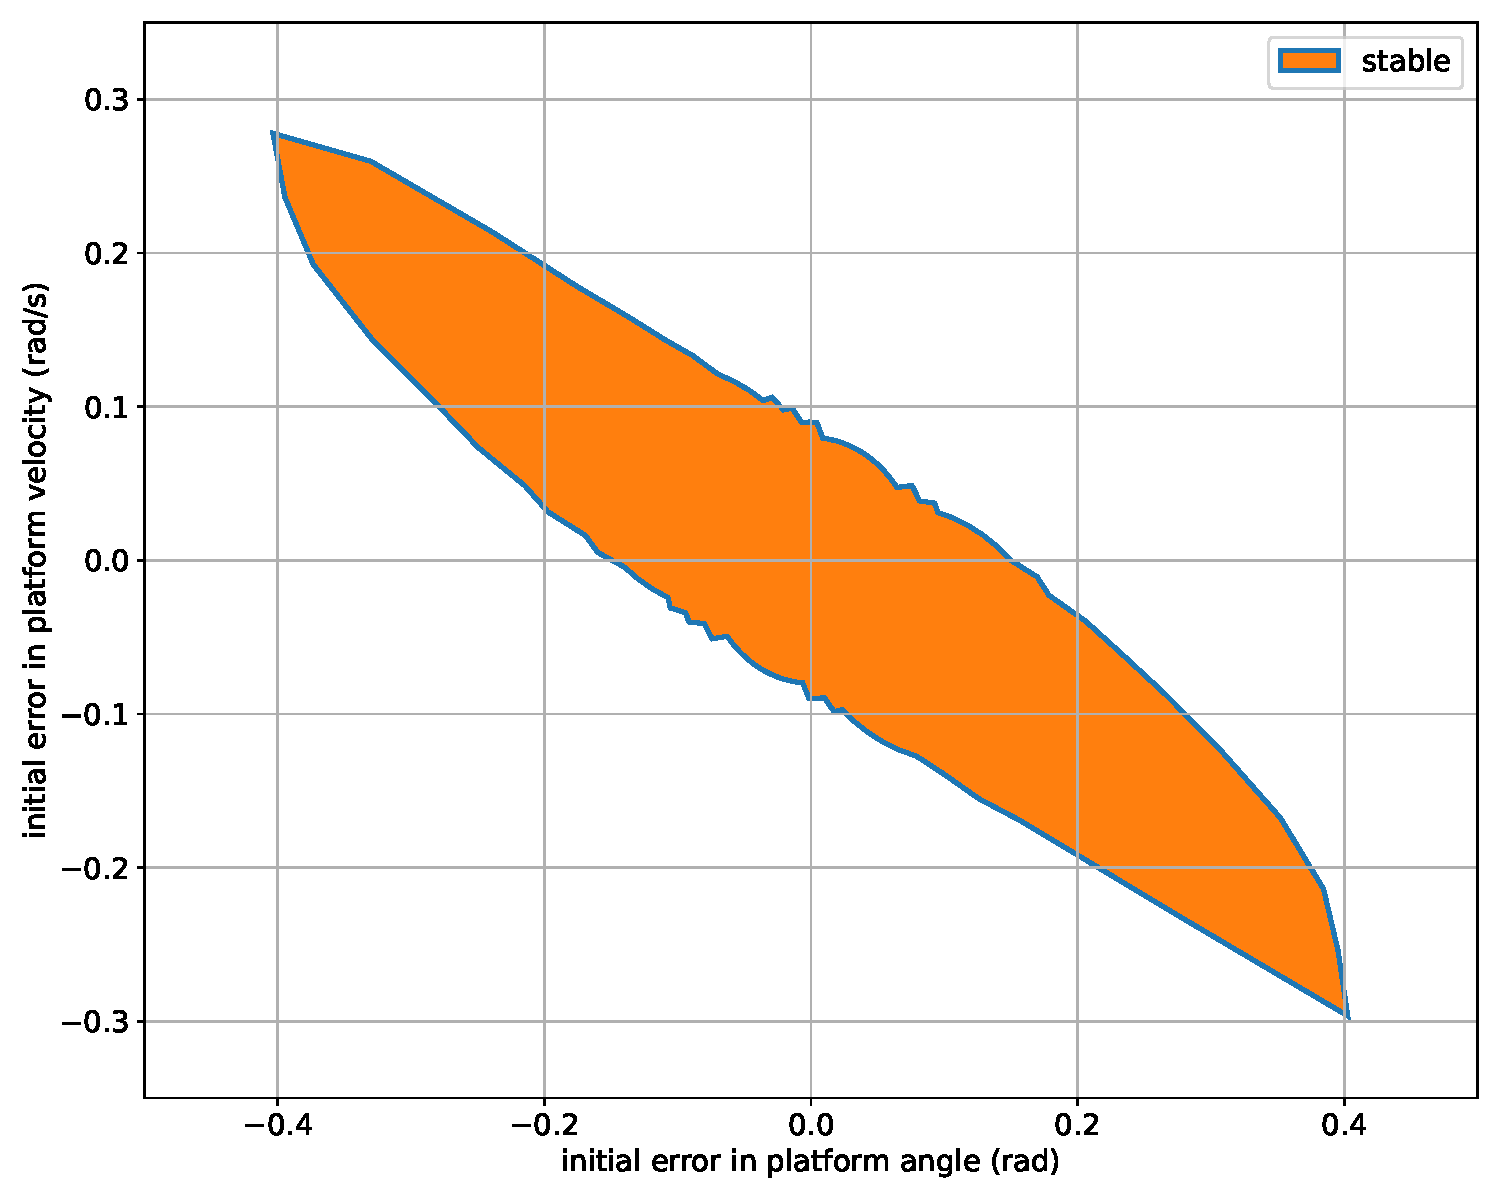
\includegraphics[width=0.6\textwidth]{fig03}
%\caption{The set of initial conditions (with zero initial error in wheel angular velocity) that produced stable closed-loop responses in simulation (i.e., for which all states converged to equilibrium within four seconds).}
%\label{fig-initial-conditions}
%\end{figure}

\begin{figure}[p]
\centering
\captionbox{A snapshot of the simulation window with the platform (light blow) and the wheel (dark blue) at an inverted configuration.\label{fig-snapshot}}
[.46\textwidth]{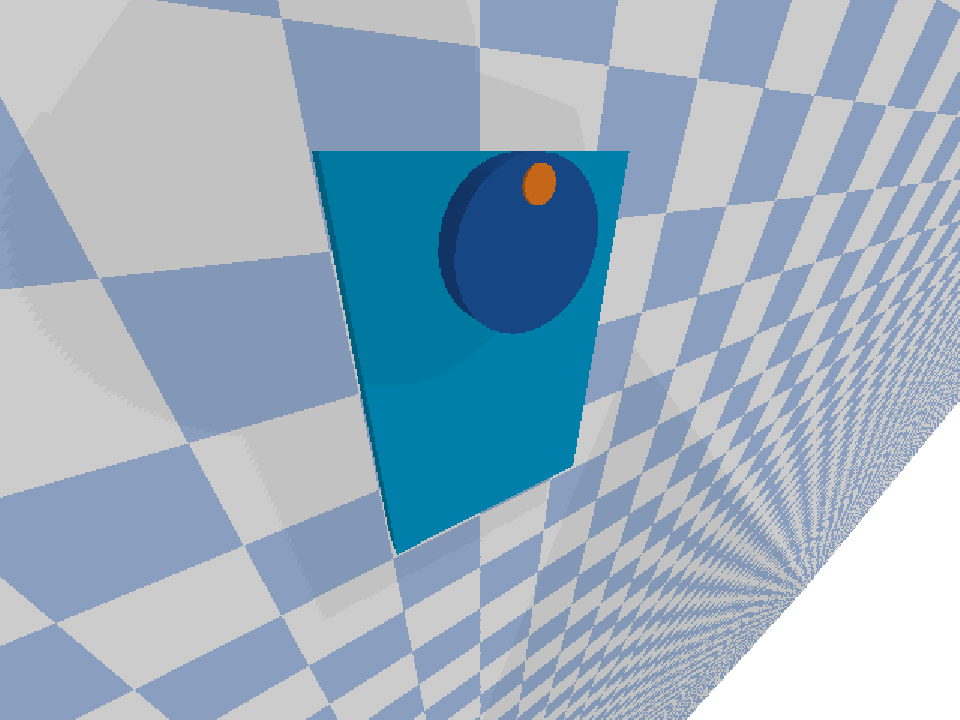
\includegraphics[height=0.375\textwidth]{fig00}}%
\hfill%
\captionbox{The set of initial conditions (with zero initial error in wheel angular velocity) that produced stable closed-loop responses in simulation (i.e., for which all states converged to equilibrium within four seconds).\label{fig-initial-conditions}}
[.46\textwidth]{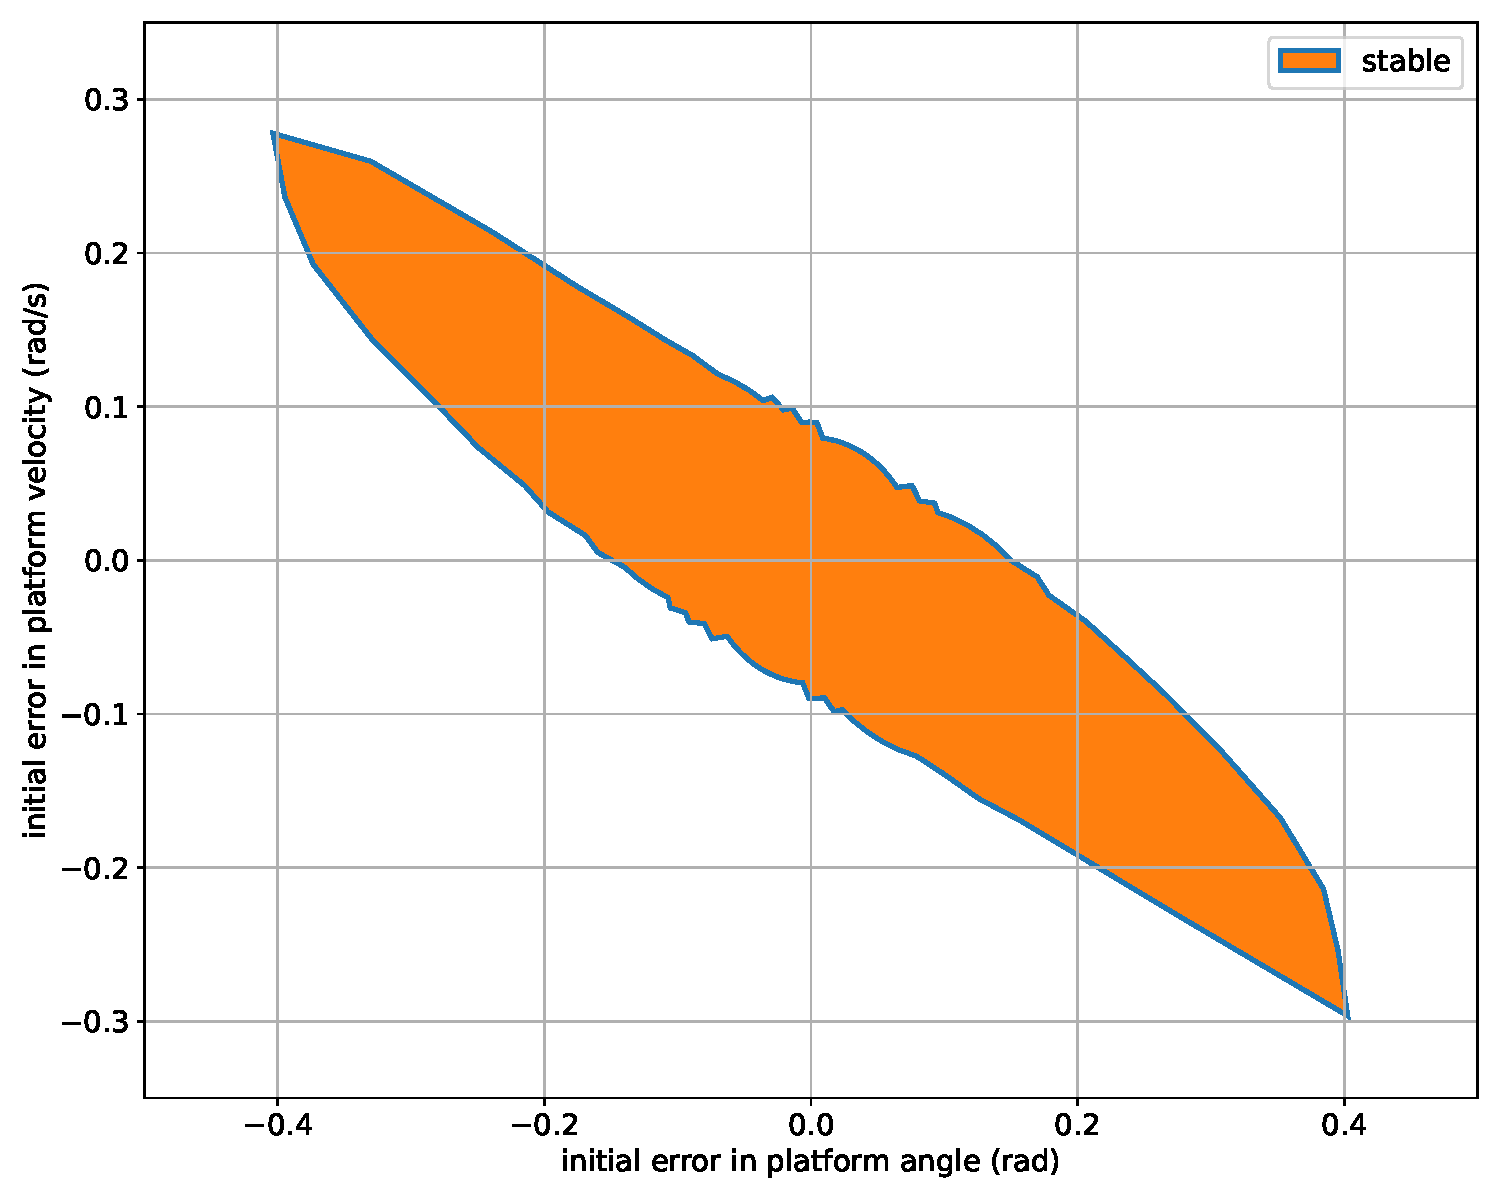
\includegraphics[height=0.375\textwidth]{fig03}}
\end{figure}


Figure \ref{fig-stable} shows the results of our experiment to find peak time and peak overshoot (Section \ref{sec-peak}), starting from the initial conditions \eqref{eq-peak-ics}.
We note that the closed-loop response is stable in this case---the platform angle, platform angular velocity, and wheel velocity all converge to equilibrium values.
The platform angle $q_{1}(t)$ exhibits a clear peak from which we computed the following peak time and peak overshoot:
\begin{equation}
T_{p} = 0.58\;\text{seconds}
\qquad\qquad
M_{p} = 0.44.
\end{equation}
Comparing these quantities to their target values \eqref{eq-peaktargets}, we see that our design produced a peak time that was nearly 30\% smaller than intended and a peak overshoot that was about 120\% larger than intended.
To rule out the possibility that errors in the linear model \eqref{eq-ss} caused this discrepancy, we also show in Figure \ref{fig-stable} the trajectory
\begin{equation}
x(t) = e^{(A - BK)t}x(0)
\end{equation}
that was predicted by this linear model. There appears to be negligible difference between what was derived from simulation and from this linear model. So, we conclude that the likely reason for not having achieved target values was the difference between our third-order linear system \eqref{eq-ss} and the canonical second-order system from which the heuristic \eqref{eq-heuristic} was derived. It is also possible that we failed to place the third eigenvalue $s_{3}$ in \eqref{eq-eigs} far enough into the left-half plane, producing a non-negligible effect on the closed-loop response.

Figure \ref{fig-initial-conditions} shows the results of our experiments to find the basin of attraction (Section \ref{sec-basin}). Again, all points inside the basin of attraction correspond to initial conditions that produced trajectories---like the one shown in Figure \ref{fig-stable} and {\em not} like the one shown in Figure \ref{fig-unstable}---satisfying the conditions \eqref{eq-stablecond} for convergence to equilibrium.
As expected, the basin of attraction contains the equilibrium point (i.e., the set of initial conditions that correspond to zero initial error in $q_{1}$, $v_{1}$, and $v_{2}$) but is {\em not} of infinite extent---initial conditions too far from equilibrium produce trajectories that do not converge.
%The boundary of the basin of attraction 
Although Fig.~\ref{fig-initial-conditions} seems to imply that the basin of attraction has a slightly uneven or noisy boundary, we suspect that this result is an artifact of the way we searched for points on the boundary (Section \ref{sec-basin}) and that the boundary would have appeared smoothed if we had increased the resolution of our search.
%However, one significant weakness of our method is that it is unable to find points in the basin of attraction 
Figure \ref{fig-initial-conditions} also seems to imply that the basin of attraction is {\em star-shaped}---that is, if
\begin{equation}
q_{1}(0) = q_{1e} + \alpha
\qquad\qquad
v_{1}(0) = v_{1e} + \beta
\qquad\qquad
v_{2}(0) = v_{2e}
\end{equation}
is in the basin of attraction, then so is
\begin{equation}
q_{1}(0) = q_{1e} + c\alpha
\qquad\qquad
v_{1}(0) = v_{1e} + c\beta
\qquad\qquad
v_{2}(0) = v_{2e}
\end{equation}
for all $c\in[0, 1]$. This conclusion, however, is likely false---our method of finding points on the boundary is {\em only} capable of producing a star-shaped inner approximation to the basin of attraction.


\section{Conclusion}
\label{sec-conclusion}

This report described our approach to design and test a controller that stabilizes a rotating platform with a reaction wheel in gravity at an inverted configuration.
Our first key result was to show that we achieved a 30\% smaller peak time and 120\% larger peak overshoot in simulation than were predicted in theory. Noting the close match between trajectories predicted by our linear model and trajectories produced by simulation, future work might focus on tuning the control design prior to implementation so that the target peak time and peak overshoot are achieved more closely.
Our second key result was to show that the closed-loop system was stable in simulation only when initial errors in platform angle and platform angular velocity were small, and to produce a star-shaped inner approximation to the basin of attraction. Future work might focus on obtaining a less conservative approximation to this basin of attraction.


\section*{Acknowledgments}

We thank the many students in the Department of Aerospace Engineering at the University of Illinois at Urbana-Champaign who have completed design projects like the one described in this report over the past decade.

\bibliography{sample}

\section*{Appendix}

The task log would appear here.



\end{document}
